\documentclass[fontsize=11pt]{article}
\usepackage{amsmath}
\usepackage[utf8]{inputenc}
\usepackage[margin=0.75in]{geometry}
\usepackage{graphicx}
\usepackage{float}
\graphicspath{{Screenshots/}}

\title{CSC110 Project Proposal: Country-wise Financial Responsibility for Climate Change}
\author{Ansh Jain, Nikhil Sreekumar, Sidharth Sachdev}
\date{Monday, December 14, 2020}

\begin{document}
    \maketitle

    \section*{2. Problem Description and Research Question}

    Change has been exponentially quick in the last century, and it certainly has not been kind to the climate of our world. Instead of guiding us away from the brink of destruction, many of our leaders have steered us right to the tipping point. Our problem is that some very privileged people are allowed to make decisions that adversely affect the entire planet. We have decided to research how various factors contribute to the individual impact of a nation on the worsening climate of the earth. We want to quantitatively find out how much each country is responsible for climate change.\newline

    Hence our research question is,

    \textbf{What is each country’s responsibility, in monetary value, towards confronting the looming climate emergency based on certain factors, ranging from the country’s effect on the earth’s climate to its fiscal ability?}\newline

    The world runs on money, and any form of commitment on a global front must start off with a budget. This resulted in us choosing a monetary approach to answer the research question. However, the aim of the project is not realized through calculating this aforementioned budget, a role imposed upon the user, but is done so by producing a fair distribution of this budget amongst the nations of the world.\newline

    We intend to go about doing so by creating a desktop application that allows the user to gain this information in whichever way is more preferable: comparing nations in a choropleth map or analyzing each country separately. It is also imperative that the application has a clean and understandable User Interface so that the user is aware of the expected input as well as the features that come with it.\newline


    A major feature of the application is providing the user with the freedom to manipulate the datasets, weightage, and factors while using a set of standard underlying equations. There is a default directory with datasets that the users can use, but they are encouraged to delete or replace them with datasets of their own before running the program. The weight of each factor, the budget, and the year of analysis can be directly altered while running the application. Together, this customizability allows for an interactive application that can produce several hypothetical budget distributions in a systematic, unbiased manner


    \section*{3. Dataset Description}

    There are two directories in which datasets are stored. 'Responsibility Datasets' is where the user enters datasets as per what best fits their idea of assigning responsibility to each nation state. 'Constant Datasets' cannot be altered by the user since they are standard values in the computational formula.


    \begin{center}
        CONSTANT DATASETS
    \end{center}

    \begin{enumerate}


        \item [1.] GDP is a dataset of the CSV format which provides basic information about each country such as GDP in from 1960 to 2017. The data has been compiled by World Bank, and OECD National Accounts.

        \item [2.]  countries\_codes\_and\_coordinates contain information regarding location and ISO 2 and 3 codes. The country name and ISO code are used. Dataset obtained from a Github repository under username Tadast.

    \end{enumerate} \newpage

    \begin{center}
        RESPONSIBILITY DATASETS (DEFAULT)
    \end{center}

    \begin{enumerate}
        \item [1.] CO2 emission is a dataset of the CSV format which provides information on the emissions of Carbon Dioxide in metric tons based on each country from 1990 to 2016. This dataset has been sourced from data.world and was created by Oak Ridge National Laboratory.

        \item [2.] Percentage use of renewable energy is a dataset of the CSV format which provides information on the percentage of renewable energy used out of the total energy consumption per country from 1960 to 2015. The dataset has been sourced from the World Bank.

        \item [3.] CRI is a dataset of the CSV format which provides information on categories such as score, fatalities, losses in millions of dollars based on the effects of climate in each country in 2014. The source of the data set is GERMANWATCH.

        \item [4.] The same GDP dataset from Constant Datasets can also serve as a factor. Thus, it is also a part of the Responsibility Datasets

    \end{enumerate}


    Note: Each Dataset provided has data for a range of years. However, the data for CRI is from the year 2014 exclusively. Hence, the only common year available to the user for analysis is 2014. The user can change this by editing the directory containing datasets as required. The user’s preference and available data may differ and they have the freedom to input datasets in their best interest. This is elaborated further in the Computational Plan.


    \section*{4. Computation}
    
    \texttt{dataset\_utilities.py} is a script that is responsible for bridging the GUI aspect of the application with the computation. \texttt{\_extract\_wanted\_column} extracts the required columns from the datasets provided, and using \texttt{name\_to\_iso}, provides a raw amalgamation of input csv files into a mapping in \texttt{raw\_datasets}. These functions are the building blocks to the following public functions that are used by other scripts.
    
    \begin{enumerate}
    	\item [1.] \texttt{map\_iso\_to\_country} creates a key-value pair of ISO code to Country dataclass. It removes all insufficient data from which a weighted average cannot be calculated. It is used to find all the countries that are to be displayed in the map.
    	
    	\item[2.] \texttt{get\_clean\_datasets} converts \texttt{map\_iso\_to\_country} back into the form of \texttt{get\_raw\_datasets}. Is important for all country related computation in \texttt{computation.py}
    	
    	\item[3.] \texttt{possible\_years} Uses the information from \texttt{get\_clean\_datasets} to return which years useful data can be derived from.
    \end{enumerate}

	The main GUI script, \texttt{user\_input.py} contains two windows in the application are built in an Object Oriented implementation, both inheriting the framework provided by \texttt{cclm\_application\_window.py}\newline

    The application first takes in user input for a year to Analyze. The user is provided a drop-down of
    possible years to choose from.\newline If the following preconditions:

    \begin{enumerate}
        \item [1.] $budget \geq \$1,000,000$
        \item [2.] Sum of all constants for weighted average $= 100$
    \end{enumerate}

	Are not satisfied, an error dialog is created.\newline

    As the application is executed, the \texttt{map\_win\_open} method in \texttt{user\_input.py} calls the \texttt{run}
    method in the script relating to map plotting, \texttt{map.py}. Method \texttt{run} is a public method that displays a choropleth map giving information about the
    budget, budget percentage, name of the country, its iso-code and each country’s data for every
    factor. This data can be viewed by hovering over the country on the map
    using the package pandas’ DataFame method to pass data into a choropleth object of \texttt{plotly.express} module that shows the map. The budget and budget percentage for each
    country are obtained by calling the private \texttt{\_plot} method that takes in the required information and passes over the values for computation in \texttt{computation.py} \newline
    
    \texttt{\_plot} calls \texttt{budget\_details} method in \texttt{computation.py} to return a dictionary mapping each country code to a
    corresponding tuple of the budget and budget percentage.\newline

    \texttt{budget\_details} is a public method that calculates the appropriate amount in US dollars to be allocated to
    each country and returns a tuple containing both budget and budget percentage for that specific country
    based on the formula,
    \[
        Budget(A) = Responsibility(A) \cdot Total \_ Budget
    \]
    \[
        GDP \% = \frac{Budget(A)}{Country's \, GDP} \cdot 100
    \]
    It does this by calling the private method \texttt{\_responsibility}. It carries out
    the major chunk of the calculation by first checking whether there is any unavailable data for a country in a
    specific factor (this is only if the country has data for at least one of the factors). If this is the
    case, then the country is removed from the dict and not displayed on the map. \newline

    \texttt{\_responsibility} also calls private methods \texttt{\_negative\_calculation} and \texttt{\_positive\_calculation} for each factor based on
    their relation of ‘direct’ or ‘inverse’ as input by the user.\newline
    \begin{enumerate}
        \item [-] if the word 'direct' is used, it means that the factor is positively correlated to climate change like
        GDP, Carbon Dioxide Emissions, and Climate Risk Index. It uses the formula,
        \[
            \frac{Country's \, \, data}{Total Data}
        \]

        \item [-] if the word 'inverse' is used, it means that the factor is negatively correlated to climate change like
        Renewable Energy.
        \[
            \frac{Total \, data - Country's \, \, data}{\displaystyle\sum_{i \in Country \, data} Total \, data - i }
        \]
    \end{enumerate}
    The result from these calculations(point out of 1) are then multiplied with the corresponding weight of the factor.
    This is done for each factor and their sum(out of 100) gives the responsibility of that country. Assuming there are 4 factors (as is in the default):
    \[
        Responsibility = \alpha F1 + \beta F2 + \gamma F3 + \delta F4
    \]
    A way to crosscheck these values
    is if the responsibilities of all countries are added, we get 100\%. Hence we know that the computation is right.
    \newline
    Using these methods, we were able to come up with an implementation for our plan and display the
    choropleth map along with the information of each country when the user hovers over that region.\newline
    All files in \texttt{qt\_designer\_automated\_scripts} are made using QtDesigner. Since they are automated,
    there implementation details are not mentioned, and they are inserted in a separate directory.
    
    \section*{5. Instructions}
    Our project works in processed datasets, hence as per the instructions, the TA must download the processed versions
    of the datasets which is a zip file named "Raw Datasets". This file should be extracted, there will be 2 folders present
    inside the extracted filed named "Constant Datasets" and "Responsibility Datasets". Constant Datasets contain 2 CSV files
    namely \texttt{countries\_code\_and\_coordinates.csv} and \texttt{GDP.csv}. These files must be inserted in the Constant Datasets
    directory directly on PyCharm. Similarly, Responsibility Datasets contain 4 CSV files namely \texttt{Carbon Dioxide Emissions.csv},
    \texttt{Climate Risk Index.csv}, \texttt{GDP.csv}, and \texttt{Renewable Energy.csv}. These files must be inserted in the Responsibility Datasets
    directory directly on PyCharm. Further instructions are also available under each directory on PyCharm in a file named \texttt{TODO\_file} which
    must be deleted once the CSV files are inserted.\newline

    \begin{figure}[H]
        \centering
        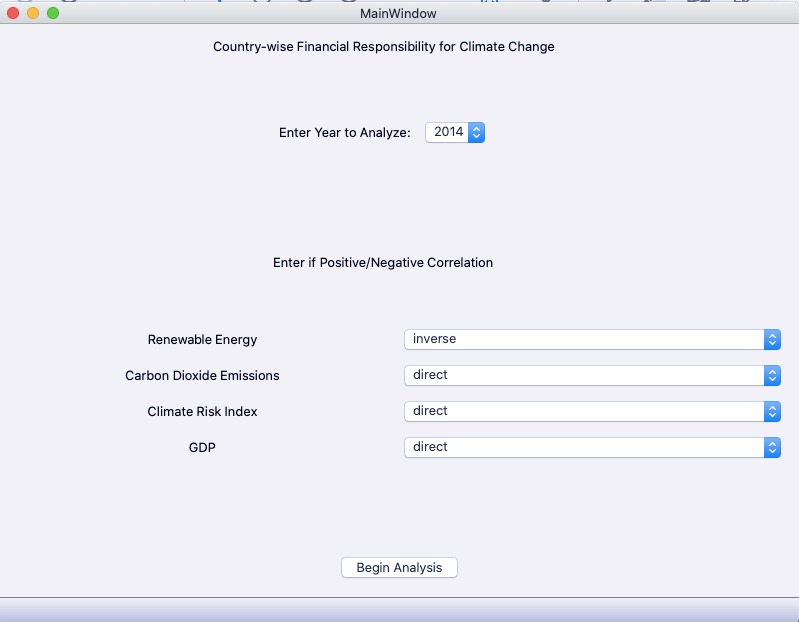
\includegraphics[width=8cm]{Figure 1.jpeg}
        \caption{GUI Screen 1}
    \end{figure}
    \begin{figure}[H]
        \centering
        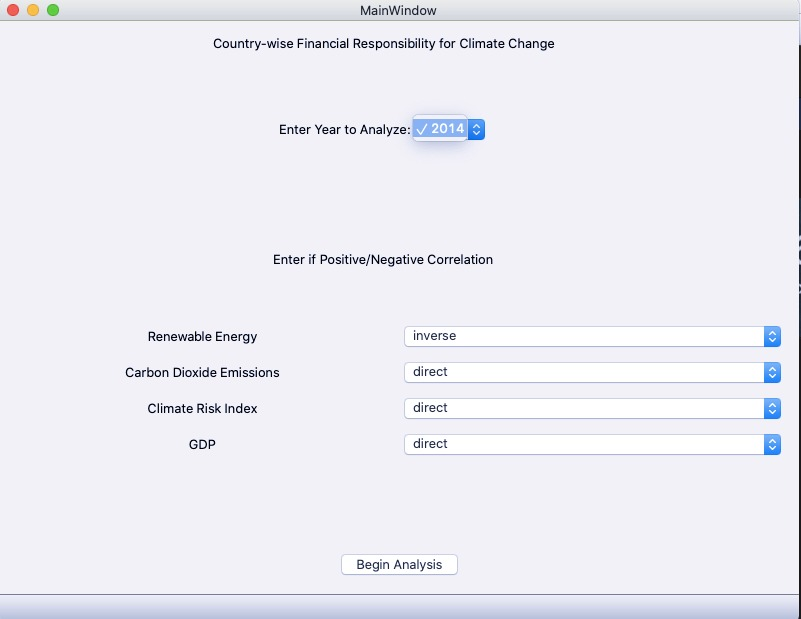
\includegraphics[width=8cm]{Figure 2.jpeg}
        \caption{Year Drop-down with CRI}
    \end{figure}
    \begin{figure}[H]
        \centering
        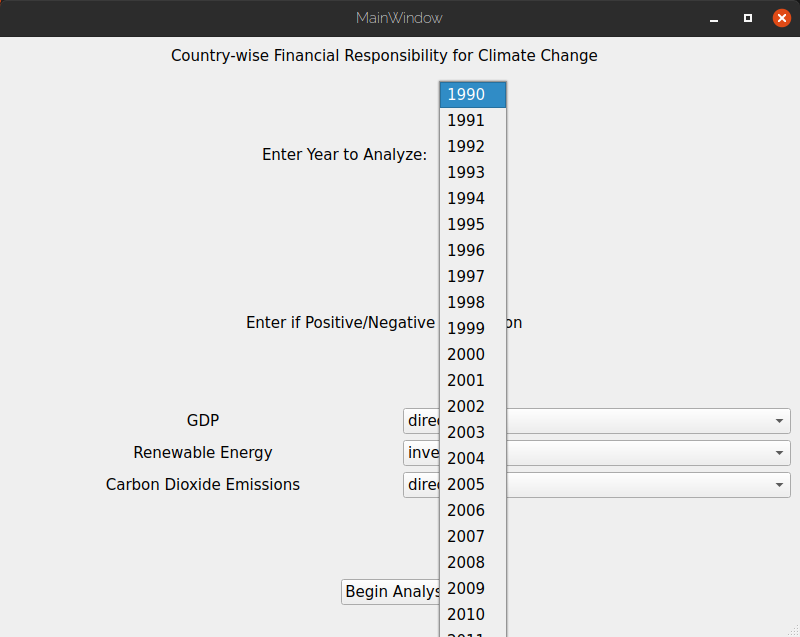
\includegraphics[width=8cm]{Figure 3.png}
        \caption{Year Drop-down without CRI}
    \end{figure}
    \begin{figure}[H]
        \centering
        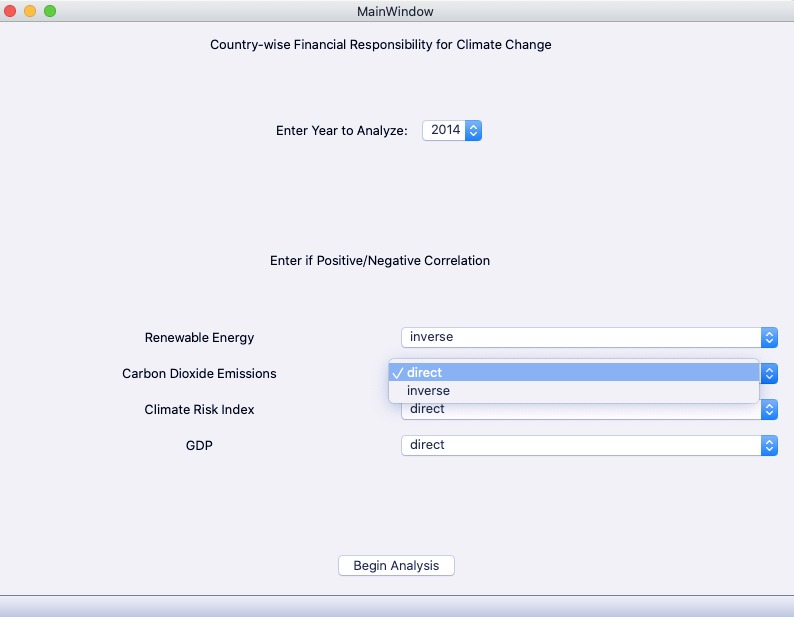
\includegraphics[width=8cm]{Figure 4.jpeg}
        \caption{Direct or Inverse Relation Drop-down}
    \end{figure}
    
    When \texttt{main.py} is run, the window that pops up is the one seen in \texttt{Figure 1}. This is the window that pops if Climate Risk Index
    is included as one of the factors with only 2014 available\texttt{(Figure 2)}. It can be seen in \texttt{Figure 3} that if the Climate Risk Index.csv was not included as one of the files
    under the Responsibility Datasets directory, numerous years are available for analysis.\newline
    The user can choose the country and choose whether he wants the factors to be directly correlated or inversely correlated
    to climate change. For the factors provided by us, the suggested relation is already set (the first option in the drop down
    menu as seen in \texttt{Figure 1}). These options can be seen in \texttt{Figure 4}\newline
    Note - Renewable Energy is recommended to have an inverse relation whereas the rest have a direct relation.\newline
    
    \begin{figure}[H]
        \centering
        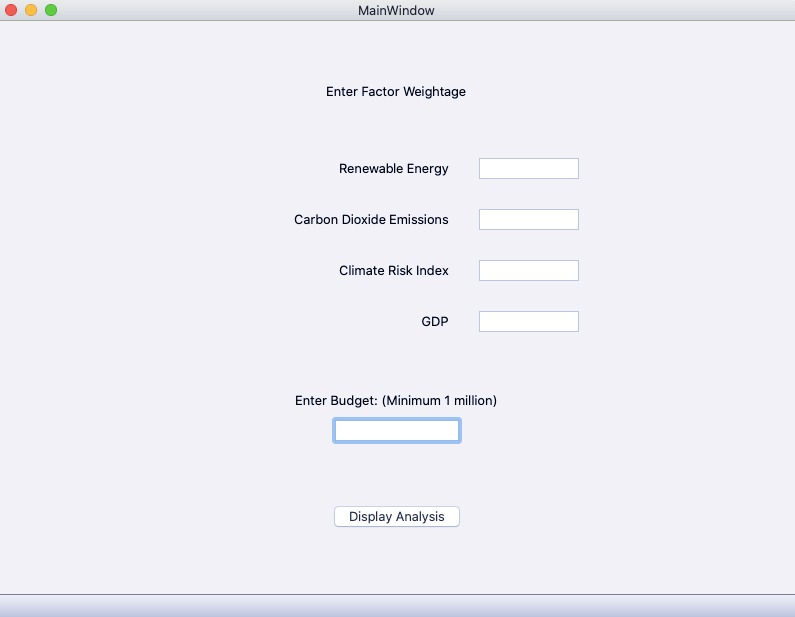
\includegraphics[width=8cm]{Figure 5.jpeg}
        \caption{GUI Screen 2}
    \end{figure}
    \begin{figure}[H]
        \centering
        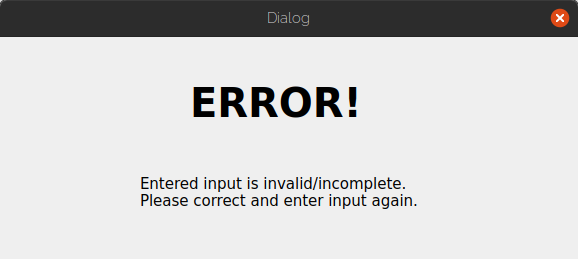
\includegraphics[width=8cm]{Figure 6.png}
        \caption{Error Message}
    \end{figure}
    
    The second window that pops up is the one seen in \texttt{Figure 4}. This screen allows the user to enter weights corresponding to
    each factor as a percentage(out of 100). It also allows the user to input the total budget which must be $\geq$ 1 million US
    dollars. If an incorrect value is entered, a window displaying "error" pops as in \texttt{Figure 5}.\newline
    
    \begin{figure}[H]
        \centering
        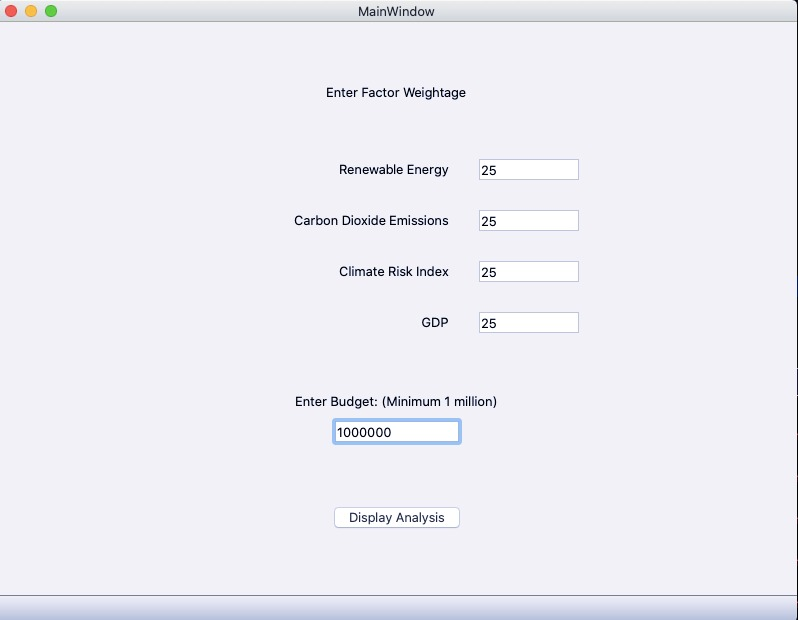
\includegraphics[width=8cm]{Figure 7.jpeg}
        \caption{Sample Data for GUI Screen 2}
    \end{figure}
    \begin{figure}[H]
        \centering
        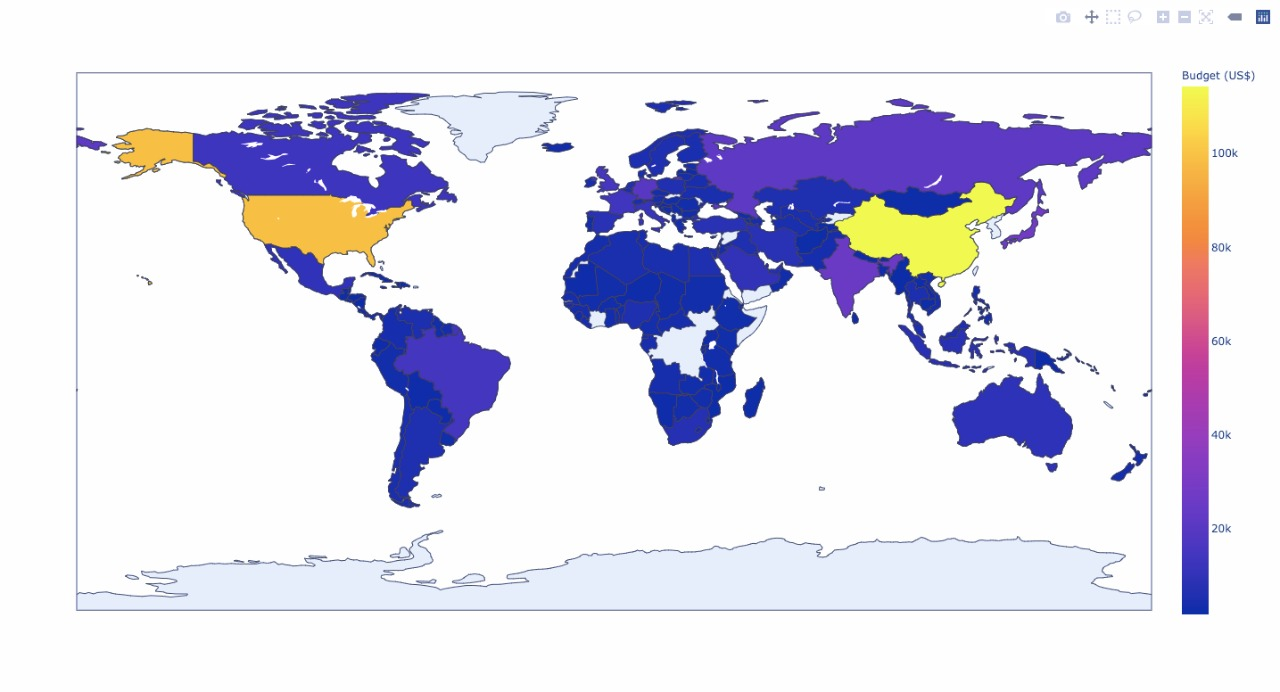
\includegraphics[width=14cm]{Figure 8.jpeg}
        \caption{Map (no hover)}
    \end{figure}
    \begin{figure}[H]
        \centering
        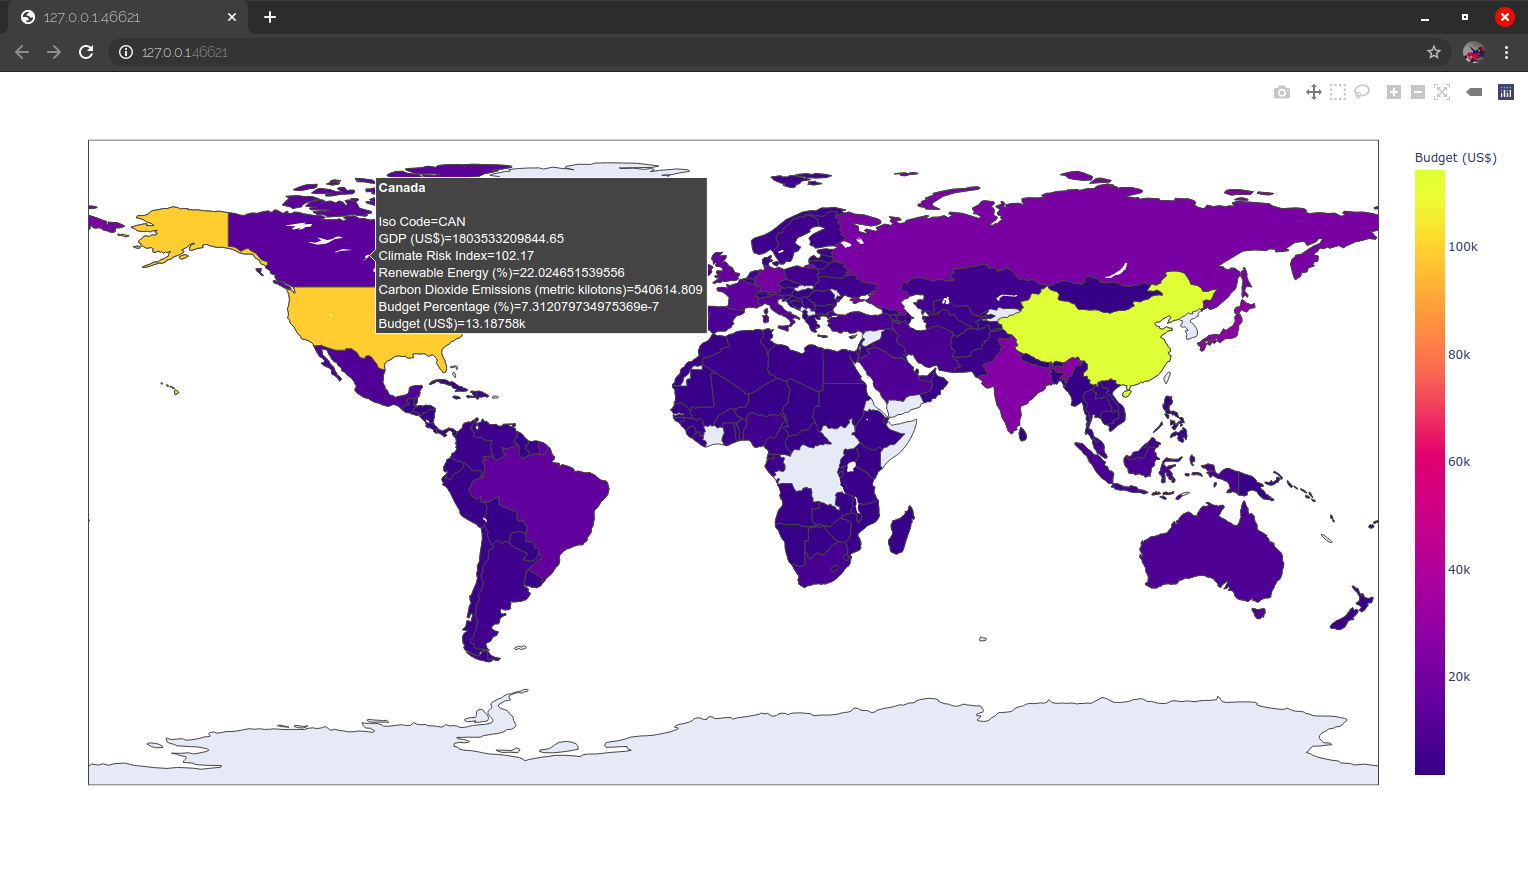
\includegraphics[width=14cm]{Figure 9.png}
        \caption{Map (hover over Canada)}
    \end{figure}
    
    We show a sample input in \texttt{Figure 7} with each factor having equal weightage of $25\%$ and the total budget
    being $1,000,000$. The map seen in \texttt{Figure 8} is displayed. When a cursor is hovered over a country, the details about
    the country like is iso-code, country name, budget, budget percentage, and the data of the factors corresponding to that
    country. This example can be seen for Canada in \texttt{Figure 9}.\newline

    \section*{6. Changes}

    As per the TA's suggestions, the changes we made to our project were:
    \begin{enumerate}
        \item [1.] Changing the project title from "Climate Change Liability Metric" to "Country-wise Financial
                    Responsibility for Climate Change".
        \item [2.] Since our project uses an equation to calculate this Financial Responsibility, we changed our
                    research question from whether a metric could be found to a more specific question of what the
                    metric is and what does it signify.
        \item [3.] Although we were suggested to use a specific region or continent to reduce the workload, we found
                    that it was easier to use all the countries since the choropleth map object under \texttt{plotly.express}
                    already contains a parameter \texttt{locations} to enter the corresponding iso-code for each country,
                    making it easier to be displayed on the map.
        \item [4.] In the dataset description of the proposal, we took different years for each of our datasets which seemed logically flawed.
                    Hence we changed our implementation of the project to include a wider range of years common to each
                    factor. Although Climate Risk Index has data only for 2014, if chosen to remove, a wider range of
                    years will be available for analysis as explained in the computation section.
    \end{enumerate}
    Apart from these fixes, our project has continued with the same plan excluding a few minor changes like correcting the
    formulas for the computation and integrating both country-wise grid and the choropleth map(our goal as per the proposal)
    into a single choropleth map. The country-wise information can be viewed by hovering over a specific country. \newline
    
    \section*{7. Discussion}
    \quad The research question led us through many formulae before we finally settled on the present mathematical model. 
    Our computational exploration helps us critically examine many aspects of the data such as determining whether a particular factor 
    has a direct or inverse relation with the required reparations, and how the choropleth map is affected by changing the weightage of each factor. 
    Although the budget percentage of each country will remain relatively stable due to the exponential but consistent decline of our climate worldwide, 
    we can also extrapolate trends over the years to predict the increase in the overall budget (since our fight against the deteriorating climate 
    becomes more and more daunting).
    \newline
    
    Let's take a look at the year 2014 when the carbon dioxide emissions, Climate Risk Index, and the gross domestic product all share 
    a direct relation with the 'climate budget' but use of renewable energy of a country has an inverse relation. Say we decide to give 
    equal weightage to each factor (25\% each) and set the budget limit as \$ 1,000,000. Now, when the application is run, the map that 
    appears displays the country-wise distribution of the total budget. By following the legend on the right side of the screen, we can 
    observe that China has the highest required climate budget (\$114,291.80) and many African nations (like Mozambique) have very low 
    budgets. Hovering over both countries, we can find out the reason for this -- China had 10,291,926.878 metric kilotons of $CO_2$ emissons 
    in 2014 while Mozambique had 8434.1 metric kilotons (around 1220 times less). Moreover, Mozambique has a renewable energy percentage 
    of 88.8570478335913\% while China only has 12.2238230065824\% and the inverse relationship between the factor and the budget 
    specifies that China should pay more to compensate for its greater impact on climate change.
    \newline
    
    Additionally, since budget percentage is a ratio between the required budget and the GDP of the country, it is possible for one 
    country to have a higher required budget than another country but a lower budget percentage due to large differences in their GDP's. 
    We see this demonstrated best in the neighbors US and Canada, where US has a required climate budget of \$98,903.30 and Canada has a 
    budget of \$13,187.58 but the US has a lower budget percentage ($5.644605277395316 \times 10^{-7}$) than Canada 
    ($7.312079734975369 \times 10^{-7}$) due to its significantly higher GDP. All these numeric and visual trends are useful in depicting 
    which country has a greater impact on the climate by calculating the required amount each country should set aside in its budget to 
    tackle the climate emergency using the different factors. 
    \newline
    
    We also ran into some unforeseen complications while working with the datasets. The data was often incomplete or missing in the 
    four datasets (representing the four factors) – many countries had gaps in data over the years and a few countries were missing 
    altogether from one or more of the chosen datasets. These cases had to be excluded from the computation. Furthermore, our model 
    relies on the user’s credibility, which means that it will unfortunately fail if the data entered is logically incorrect. 
    For example, a reverse relationship between a factor and the budget (direct instead of inverse or vice versa) would result in 
    unbalanced reparations and some countries that should pay more might end up paying less. To deepen our bounds of exploration in the future, 
    we would like to give the user more datasets (and therefore factors) to include in the budget computation of each country 
    and also offer the user a clearer choice when selecting inputs. The user would be able to 'keep' or 'remove' the factors through a drop-down menu. 
    The application's default datasets chosen by us (such as the four factors) would have fixed relations (direct or indirect) 
    and the user would have to correctly specify the relation for any new datasets that they add. Another visual that we would include 
    in the application is a graph that plots a chosen country’s data over the years and extrapolates the line graph to predict the budget in future years.
    \newline
    
    Overall, Country-wise Financial Responsibility for Climate Change is a useful application that achieves success in its goal 
    to obtain a realistic monetary metric. Its interactive interface provides 
    the user with insight into the international responsibility of each nation in combating the climate emergency. By having a visual representation 
    of the choropleth map side by side with numeric data, the user can perceive trends compactly and distinctly. Thus, our research question 
    propels the climate change conversation towards a possible solution by assigning a fiscal benchmark and will hopefully 
    help provide impetus to reformative action.
    \newline

    \newpage

    \section*{8. References}

    \begin{enumerate}
    	\item[1.] “Qt Documentation.” Qt for Python - Qt for Python, doc.qt.io/qtforpython/.

    	 \item[2.] “Choropleth Maps.” Plotly, plotly.com/python/choropleth-maps/.

    	 \item[3.] Oak Ridge National Laboratory. CO2 Emssions (Kt), data.worldbank.org/indicator/EN.ATM.CO2E.KT.

    	 \item[4.] “Renewable Energy Consumption
    	 (\% of Total Final Energy Consumption).” Data,\newline data.worldbank.org/indicator/EG.FEC.RNEW.ZS.

    	 \item[5.] Eckstein, David. “Global Climate Risk Index 2014.” Germanwatch.org, https://germanwatch.org/en/7659.

    	 \item[6.] World Bank, and OECD National Accounts. “GDP (Current US\$).”

    	  Data, n.d. https://data.worldbank.org/indicator/NY.GDP.MKTP.CD.

    	 \item[7.] Tamošauskas, Tadas. “Countries with Their (ISO 3166-1) Alpha-2 Code, Alpha-3 Code, UN M49, Average Latitude and Longitude Coordinates.” Gist. Accessed December 14, 2020. https://gist.github.com/tadast/8827699.
    \end{enumerate}


\end{document}
